\documentclass[
  11pt,
  letterpaper,
   addpoints,
   answers
  ]{exam}

\usepackage{../exercise-preamble}

\begin{document}

\noindent
\begin{minipage}{0.47\textwidth}

\includegraphics[width=\textwidth]{../fcfm_die}
\end{minipage}
\begin{minipage}{0.53\textwidth}
\begin{center} 
\large\textbf{Electromagnetismo Aplicado} (EL3103-1) \\
\large\textbf{Clase auxiliar 8} \\
\normalsize Prof.~Benjamin Jacard H.\\
\normalsize Prof.~Aux.~Erik Saez A.
\end{center}
\end{minipage}



\vspace{0.5cm}
\noindent
\vspace{.85cm}
\begin{questions}
    %%%%%%%%%%%%%%%%%%%%%%%%%%%%
    \question Para una guia de onda general encuentre las expresiones que caracterizan tanto las ondas TM y TE.
  \begin{center}
        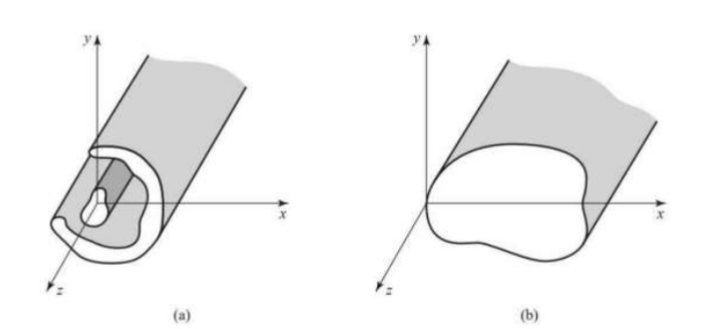
\includegraphics[width=0.5\textwidth]{Auxiliar_8_1}
        \captionof{figure}{Esquema de la linea de transmisión}
      \end{center}
    %%%%%%%%%%%%%%%%%%%%%%%%%%%
    \begin{solution}
        Buscamos obtener las expresiones que caracterizan tanto las ondas TM y TE, sabemos además que la principal diferencia entre las ondas TEM, TE y TM, radica en la dirección de propagación:

\begin{center}
    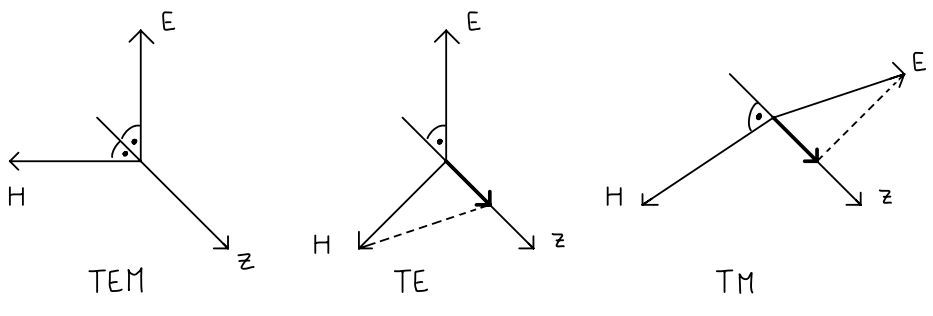
\includegraphics[width=0.8\textwidth]{Auxiliar_8_2}
\end{center}

En las ondas TE (Transversales Eléctricas), no existe una componente longitudinal del campo eléctrico en la dirección de propagación, es decir, $E_z = 0$. Sin embargo, el campo magnético puede tener una componente en esa dirección, por lo que $H_z \neq 0$. En las ondas TM (Transversales Magnéticas), no existe una componente longitudinal del campo magnético en la dirección de propagación, es decir, $H_z = 0$. En este caso, el campo eléctrico sí presenta una componente en esa dirección, por lo que $E_z \neq 0$.

\begin{align}
    \vec{E}(x, y, z) &= [\vec{e}(x, y) + \hat{z}e_z(x, y)]e^{j\beta z} \tag{1}\\
    \vec{H}(x, y, z) &= [\vec{h}(x, y) + \hat{z}h_z(x, y)]e^{j\beta z} \tag{2}
\end{align}

Donde tenemos que $\vec{e}$ y $\vec{h}$ corresponden a los campos transversales ($\hat{x}$ y $\hat{y}$), por contraparte $e_z$ y $h_z$ representan los campos longitudinales ($\hat{z}$). Sabemos de las ecuaciones de Maxwell-Heaviside que:

\begin{align}
    \nabla \times \vec{E} &= -j\omega\mu \vec{H} \tag{3} \\
    \nabla \times \vec{H} &= j\omega\epsilon \vec{E} \tag{4}
\end{align}

Como estamos considerando las ecuaciones generales luego se pueden desplazar en todas las direcciones por lo que se tiene que:

\begin{equation}
    \begin{vmatrix}
        \hat{i} & \hat{j} & \hat{k} \\
        \frac{\partial}{\partial x} & \frac{\partial}{\partial y} & \frac{\partial}{\partial z} \\
        E_x & E_y & E_z
    \end{vmatrix}
    = -j\omega\mu (H_x\hat{x} + H_y\hat{y} + H_z\hat{z})
    \tag{5}
\end{equation}

Con lo que obtenemos el siguiente set de ecuaciones para la ecuación (3):

\begin{align}
    \frac{\partial E_z}{\partial y} - \frac{\partial E_y}{\partial z} &= -j\omega\mu H_x \tag{6} \\
    \frac{\partial E_x}{\partial z} - \frac{\partial E_z}{\partial x} &= -j\omega\mu H_y \tag{7} \\
    \frac{\partial E_y}{\partial x} - \frac{\partial E_x}{\partial y} &= -j\omega\mu H_z \tag{8}
\end{align}

Análogamente para la ecuación (4) se obtienen el siguiente set de ecuaciones:

\begin{align}
    \frac{\partial H_z}{\partial y} - \frac{\partial H_y}{\partial z} &= j\omega\epsilon E_x \tag{9} \\
    \frac{\partial H_x}{\partial z} - \frac{\partial H_z}{\partial x} &= j\omega\epsilon E_y \tag{10} \\
    \frac{\partial H_y}{\partial x} - \frac{\partial H_x}{\partial y} &= j\omega\epsilon E_z \tag{11}
\end{align}

Dado que buscamos obtener caracterizaciones sobre las direcciones $E_z$ y $H_z$ (Para posteriormente analizar las ondas TE y TM) luego dejamos las expresiones anterior en función de estas, con lo que se obtiene el siguiente set de ecuaciones:

\begin{align}
    H_x &= \frac{j}{k_c^2} \left(\omega\epsilon \frac{\partial E_z}{\partial y} - \beta \frac{\partial H_z}{\partial x} \right) \tag{12}\\
    H_y &= -\frac{j}{k_c^2} \left(\omega\epsilon \frac{\partial E_z}{\partial x} - \beta \frac{\partial H_z}{\partial y} \right) \tag{13}\\
    E_x &= -\frac{j}{k_c^2} \left( \beta \frac{\partial E_z}{\partial x} + \omega\mu \frac{\partial H_z}{\partial y} \right) \tag{14}\\
    E_y &= \frac{j}{k_c^2} \left( -\beta \frac{\partial E_z}{\partial y} + \omega\mu \frac{\partial H_z}{\partial x} \right) \tag{15}
\end{align}

Donde se tendrá que $k_c = k^2 - \beta^2$ la cual se denominará como frecuencia de corte y es un parámetro muy importante en temas de diseño y análisis. Una vez obtenidas las expresiones analizaremos los casos particulares para ondas TE y TM.

\textbf{Caso Ondas TE}

Sabemos que en este tipo de ondas tenemos que $E_z = 0$, con lo que debido a esto nuestras ecuaciones se reducen a lo siguiente:

\begin{align}
    H_x &= -\frac{j\beta}{k_c^2} \frac{\partial H_z}{\partial x} \tag{16}\\
    H_y &= -\frac{j\beta}{k_c^2} \frac{\partial H_z}{\partial y} \tag{17}\\
    E_x &= -\frac{j\omega\mu}{k_c^2} \frac{\partial H_z}{\partial y} \tag{18}\\
    E_y &= \frac{j\omega\mu}{k_c^2} \frac{\partial H_z}{\partial x} \tag{19}
\end{align}

Con lo que podemos reducir las ecuaciones a lo siguiente:

\begin{equation}
    \left( \frac{\partial^2}{\partial x^2} + \frac{\partial^2}{\partial y^2} + k_c^2 \right) H_z = 0 \tag{20}
\end{equation}

Ecuación general para ondas TE que puede utilizarse para cualquier tipo de geometría.

\textbf{Caso Ondas TM}

En este tipo de ondas sabemos que $H_z = 0$ por lo que el desarrollo es análogo a lo anterior obteniendo el siguiente set de ecuaciones:

\begin{align}
    H_x &= \frac{j\omega\epsilon}{k_c^2} \frac{\partial E_z}{\partial y} \tag{21}\\
    H_y &= -\frac{j\omega\epsilon}{k_c^2} \frac{\partial E_z}{\partial x} \tag{22}\\
    E_x &= -\frac{j\beta}{k_c^2} \frac{\partial E_z}{\partial x} \tag{23}\\
    E_y &= -\frac{j\beta}{k_c^2} \frac{\partial E_z}{\partial y} \tag{24}
\end{align}

Luego podemos expresar de manera general la expresión como:

\begin{equation}
    \left( \frac{\partial^2}{\partial x^2} + \frac{\partial^2}{\partial y^2} + k_c^2 \right) E_z = 0 \tag{25}
\end{equation}

Con lo que se obtienen las ecuaciones general para las ondas TE y TM.

    \end{solution}
    %%%%%%%%%%%%%%%%%%%%%%%%%%%%
    \question  Sea el caso particular de una guia de onda rectangular, en base a las expresiones obtenidas con anterioridad encuentre la caracterizacion de esta configuracion (Considerando las ecuaciones de borde vistas en la figura.)
    \begin{center}
        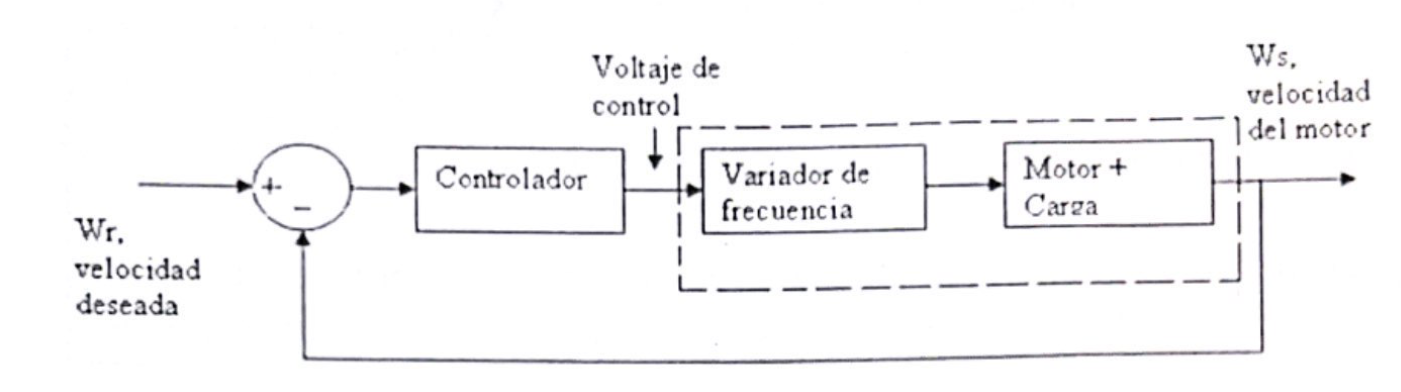
\includegraphics[width=0.45\textwidth]{Auxiliar_8_3}
        \captionof{figure}{Guia de onda rectangular y sus CB}
      \end{center}
    %%%%%%%%%%%%%%%%%%%%%%%%%%%%
    \begin{solution}
        Dado que buscamos caracterizar para una guía de onda rectangular, se tiene lo siguiente:

\begin{center}
    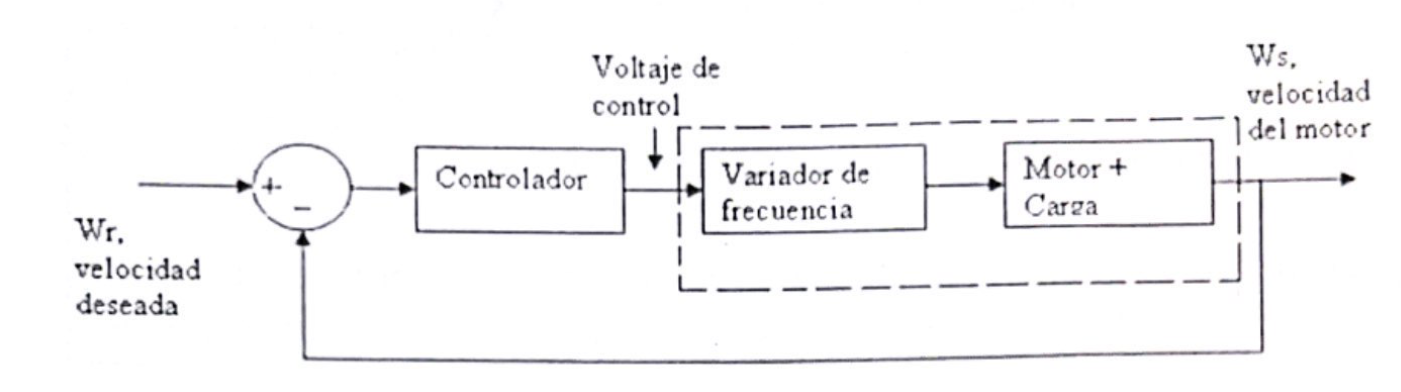
\includegraphics[width=0.5\textwidth]{Auxiliar_8_3}
\end{center}

Donde se debe asumir que $a > b$, además dado que asumimos que estamos trabajando con un conductor lo suficientemente bueno $\sigma \to \infty$ luego en las paredes del conductor no habrá campo eléctrico y por tanto tenemos las siguientes condiciones de borde:
\begin{align}
    e_x(x, y) = 0 \quad &\text{(En $y=0$, $y=b$)} \tag{26} \\
    e_y(x, y) = 0 \quad &\text{(En $x=0$, $x=a$)} \tag{27}
\end{align}

Luego analizaremos el problema para los dos tipos de ondas que se propagan, es decir TM y TE, dado que no existe una diferencia de potencial para que se tenga presencia de ondas TEM, por tanto:

\textbf{Caso 1 Ondas TM}

Sea la siguiente ecuación que obtuvimos antes:
\begin{equation}
    \left( \frac{\partial^2}{\partial x^2} + \frac{\partial^2}{\partial y^2} + k_c^2 \right) E_z = 0 \tag{28}
\end{equation}

En base a lo anterior tendremos que la componente $E_z$ será función solo de $x$ e $y$, lo interesante de esto es que permitirá el uso del método de separación de variables, tal que:
\begin{equation}
    E_z(x, y) = X(x)Y(y) = XY \tag{29}
\end{equation}

Reescribiendo la ecuación se tiene:
\begin{equation}
    \left( \frac{\partial^2}{\partial x^2} + \frac{\partial^2}{\partial y^2} + k_c^2 \right) E_z = 0 \tag{30}
\end{equation}
\begin{equation}
    \left( \frac{\partial^2}{\partial x^2} + \frac{\partial^2}{\partial y^2} + k_c^2 \right) XY = 0 \tag{31}
\end{equation}
\begin{equation}
    Y \frac{\partial^2 X}{\partial x^2} + X \frac{\partial^2 Y}{\partial y^2} + k_c^2 XY = 0 \tag{32}
\end{equation}

Dividiendo la expresión por $\frac{1}{XY}$ se tiene:
\begin{equation}
    \frac{1}{X}\frac{\partial^2 X}{\partial x^2} + \frac{1}{Y}\frac{\partial^2 Y}{\partial y^2} + k_c^2 = 0 \tag{33}
\end{equation}

La expresión $k_c^2$ vendrá dada por lo siguiente $k_c^2 = k_x^2 + k_y^2$ por lo que separando por componente:
\begin{align}
    \frac{\partial^2 X}{\partial x^2} + k_x^2 X = 0 \tag{34} \\
    \frac{\partial^2 Y}{\partial y^2} + k_y^2 Y = 0
\end{align}

Luego se puede resolver cada ecuación por separado dando como resultado lo siguiente:
\begin{align}
    x &= A \cos(k_x x) + B \sin(k_x x) \\
    y &= C \cos(k_y y) + D \sin(k_y y) \tag{35}
\end{align}

Dado que previamente definimos $E_z = X(x)Y(y)$ asumiendo que depende independientemente de estas dos componentes, obtenemos que el campo vendrá dado por:
\begin{equation}
    E_z = (A \cos(k_x x) + B \sin(k_x x))(C \cos(k_y y) + D \sin(k_y y)) \tag{36}
\end{equation}

Con lo que debemos despejar las constantes $A, B, C, D$, por lo que utilizaremos las condiciones de borde definidas previamente, con lo que se tiene:
\begin{align}
    E_z = 0 = (A \cos(k_x 0) + B \sin(k_x 0))(C \cos(k_y y) + D \sin(k_y y)) \tag{37} \\
    = A(C \cos(k_y y) + D \sin(k_y y)) = 0 \tag{38}
\end{align}

Como buscamos una solución no trivial, se impondrá que $A = 0$ (obteniendo el valor de la primera variable), análogamente si evaluamos en $y = 0$ tendremos que:
\begin{align}
    E_z = 0 = (B \sin(k_x x))(C \cos(k_y \cdot 0) + D \sin(k_y \cdot 0)) \\
    = C(B \sin(k_x x)) = 0 \tag{40}
\end{align}

Con lo que nuevamente para no obtener soluciones triviales se impone que $C = 0$, con esto obtenemos otra incógnita más, luego tenemos que el campo $E_z$ se reduce a:
\begin{equation}
    E_z = B \sin(k_x x) D \sin(k_y y) \tag{41}
\end{equation}

Luego evaluando sobre las dos condiciones de borde restantes tenemos que:
\begin{equation}
    E_z = 0 = B \sin(k_x a) D \sin(k_y y) \qquad (\text{Para } x=a) \tag{42}
\end{equation}

Nos despreocupáramos de la variable $y$, dado que nos interesa análisis solo los valores asociados a $x$, y por tanto se tiene que:
\begin{align}
    E_z = B \sin(k_x a) = 0 \tag{43} \\
    \sin(k_x a) = 0 \tag{44} \\
    k_x a = m\pi \tag{45} \\
    k_x = \frac{m\pi}{a} \tag{46}
\end{align}

De esta manera obtenemos una expresión asociada a $k_x$, análogamente para $k_y$ tenemos que:
\begin{align}
    E_z = D \sin(k_y b) = 0 \tag{47} \\
    \sin(k_y b) = 0 \tag{48} \\
    k_y b = n\pi \tag{49} \\
    k_y = \frac{n\pi}{b} \tag{50}
\end{align}

Una vez encontrado todas las expresiones, tenemos que el campo eléctrico vendrá expresado por:
\begin{align}
    E_z &= B \sin(k_x x) \sin(k_y y) \tag{51} \\
        &= B \sin\left(\frac{m\pi x}{a}\right) \sin\left(\frac{n\pi y}{b}\right) e^{-j\beta z} \tag{52} \\
        &= \beta_{mn} \sin\left(\frac{m\pi x}{a}\right) \sin\left(\frac{n\pi y}{b}\right) e^{-j\beta z} \tag{53}
\end{align}

Donde se tiene que $BD = \beta_{mn}$, estos valores usualmente se encuentran tabulados en tablas para los diferentes guías que utilizamos (Dado que rara vez tendremos una geometría con la que no estén tabulados dichos valores). El resultado final nos dice como se propaga la onda en la dirección de propagación.

Finalmente se obtiene una expresión general para $k_c$ la cual vendrá dada por:
\begin{equation}
    k_c^2 = k_x^2 + k_y^2 = \left(\frac{m\pi}{a}\right)^2 + \left(\frac{n\pi}{b}\right)^2 \tag{54}
\end{equation}

Luego para encontrar la denominada frecuencia de corte podemos realizar el siguiente arreglo respecto a lo último:
\begin{equation}
    k_c = \frac{2\pi}{\lambda_c} = \frac{2\pi}{\nu / f_c} = \frac{2\pi f_c}{\nu} = \frac{w_c}{\nu} = w_c \sqrt{\mu\epsilon}
\end{equation}

Recordemos que podemos expresar la velocidad en un medio como $\nu = \frac{1}{\sqrt{\mu\epsilon}}$, de esta manera tenemos que la frecuencia de corte vendrá dada por:
\begin{align}
    (w_c \sqrt{\mu\epsilon})^2 &= \left( \frac{m\pi}{a} \right)^2 + \left( \frac{n\pi}{b} \right)^2 \tag{56} \\
    w_c &= \frac{1}{\mu\epsilon} \sqrt{\left( \frac{m\pi}{a} \right)^2 + \left( \frac{n\pi}{b} \right)^2} \tag{57} \\
    f_c &= \frac{1}{2\pi\mu\epsilon} \sqrt{\left( \frac{m\pi}{a} \right)^2 + \left( \frac{n\pi}{b} \right)^2} \tag{58} \\
    f_c &= \frac{c}{2\pi \sqrt{\mu_r \epsilon_r}} \sqrt{\left( \frac{m\pi}{a} \right)^2 + \left( \frac{n\pi}{b} \right)^2} \tag{59}
\end{align}

Podemos dejarlo en función de las constantes relativas de igual manera. Es importante notar que la frecuencia de corte dependerá tanto de $m$ y $n$, es por esto que el orden en este tipo de ondas es Súper importante, esto dado que no será lo mismo una frecuencia de corte $f_{10}$ que $f_{01}$, es por esto que el orden que impusimos anteriormente que $a > b$ se debe mantener, así como el orden de los subíndices! En el contexto en el que trabajamos podemos expresar la constante de propagación $\beta$:
\begin{align}
    \beta^2 &= k^2 - k_c^2 \tag{60} \\
    \beta^2 &= k^2 - \left[ \left( \frac{m\pi}{a} \right)^2 + \left( \frac{n\pi}{b} \right)^2 \right] \tag{61}
\end{align}

Donde $k$ representa el número de onda, luego esto nos dice que existirá propagación ssi se tiene que $k > k_c$ por eso no todas las ondas se transmitirán al mismo tiempo y dependerán de los valores de $m$ y $n$ que utilicemos que modifican el valor de $k_c$, finalmente dado que buscábamos obtener las expresiones de los campos se tendrá que reemplazando el valor de $E_z$:

\begin{align}
    H_x = \frac{j\omega\epsilon}{k_c^2} \frac{\partial E_z}{\partial y}
    &\Rightarrow
    E_x = -\frac{j\beta m\pi}{a k_c^2} B_{mn} \cos\left(\frac{m\pi x}{a}\right)\sin\left(\frac{n\pi y}{b}\right) e^{-j\beta z} \tag{62} \\
    H_y = -\frac{j\omega\epsilon}{k_c^2} \frac{\partial E_z}{\partial x}
    &\Rightarrow
    E_y = -\frac{j\beta n\pi}{b k_c^2} B_{mn} \sin\left(\frac{m\pi x}{a}\right)\cos\left(\frac{n\pi y}{b}\right) e^{-j\beta z} \tag{63} \\
    E_x = -\frac{j\beta}{k_c^2} \frac{\partial E_z}{\partial x}
    &\Rightarrow
    H_x = -\frac{j\omega\epsilon n\pi}{k_c^2 b} B_{mn} \sin\left(\frac{m\pi x}{a}\right)\cos\left(\frac{n\pi y}{b}\right) e^{-j\beta z} \tag{64} \\
    E_y = -\frac{j\beta}{k_c^2} \frac{\partial E_z}{\partial y}
    &\Rightarrow
    H_y = \frac{j\omega\epsilon m\pi}{k_c^2 a} B_{mn} \cos\left(\frac{m\pi x}{a}\right)\sin\left(\frac{n\pi y}{b}\right) e^{-j\beta z} \tag{65}
\end{align}

Con lo que finalmente se obtiene la expresión buscada.

\textbf{Caso 2 Ondas TE}

El procedimiento para obtener las ecuaciones que caracterizan estas ondas es análogo al anterior con lo que se obtiene que:
\begin{equation}
    H_z = A_{mn} \cos\left(\frac{m\pi x}{a}\right)\cos\left(\frac{n\pi y}{b}\right)e^{-j\beta z} \tag{66}
\end{equation}

Con lo que reemplazando en el set de ecuaciones se tiene que:
\begin{align}
    H_x = -\frac{j\beta}{k_c^2} \frac{\partial H_z}{\partial x}
    &\Rightarrow
    H_x = \frac{j\beta m\pi}{k_c^2 a} A_{mn} \sin\left(\frac{m\pi x}{a}\right)\cos\left(\frac{n\pi y}{b}\right) e^{-j\beta z} \tag{67} \\
    H_y = -\frac{j\beta}{k_c^2} \frac{\partial H_z}{\partial y}
    &\Rightarrow
    H_y = \frac{j\beta n\pi}{k_c^2 b} A_{mn} \cos\left(\frac{m\pi x}{a}\right)\sin\left(\frac{n\pi y}{b}\right) e^{-j\beta z} \tag{68} \\
    E_x = -\frac{j\omega\mu}{k_c^2} \frac{\partial H_z}{\partial y}
    &\Rightarrow
    E_x = \frac{j\omega\mu n\pi}{k_c^2 b} A_{mn} \cos\left(\frac{m\pi x}{a}\right)\sin\left(\frac{n\pi y}{b}\right) e^{-j\beta z} \tag{69} \\
    E_y = \frac{j\omega\mu}{k_c^2} \frac{\partial H_z}{\partial x}
    &\Rightarrow
    E_y = -\frac{j\omega\mu m\pi}{k_c^2 a} A_{mn} \sin\left(\frac{m\pi x}{a}\right)\cos\left(\frac{n\pi y}{b}\right) e^{-j\beta z} \tag{70}
\end{align}

Donde se tiene que el modo dominante de una onda será la $TE_{01}$, es decir, el primero que se propagará en la guía de onda rectangular. Es importante notar que si bien la frecuencia de corte para ambos modos es igual, luego no se transmitirán todas a la misma frecuencia, esto debido a las distribuciones de los campos, es por esto que el orden aproximado es el siguiente:

\begin{center}
    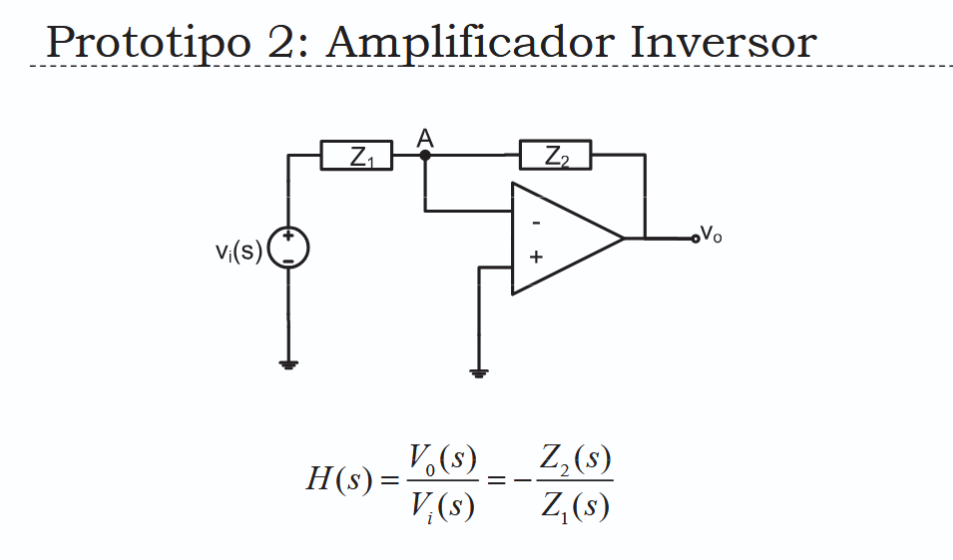
\includegraphics[width=0.7\textwidth]{Auxiliar_8_4}
\end{center}

    \end{solution}
%%%%%%%%%%%%%%%%%%%%%%%%%%%%
\question Se tiene una guía de ondas común, compuesta de dimensiones rectangulares $a = 2.29\,\text{cm}$ y $b = 1.02\,\text{cm}$, y con aire como dieléctrico. Entonces determine la frecuencia de corte, $v_{\text{cutoff},mn}$ para el modo más bajo, TM$_{11}$, y para los modos TM$_{12}$ y TM$_{21}$. Además, determine $\eta_{\text{TM},11}$, $\beta_{11}$, $u_{11}$, y $\lambda_{11}$ para el modo TM$_{11}$ a una frecuencia de $18\,\text{GHz}$.
%%%%%%%%%%%%%%%%%%%%%%%%%%%%%%%%
\begin{solution}
    \begin{equation}
    f_{cm,n} = \frac{c}{2} \sqrt{\left(\frac{m}{a}\right)^2 + \left(\frac{n}{b}\right)^2} \tag{71}
\end{equation}

donde $m$ y $n$ son los modos de la guía de ondas. Evaluamos para los modos TM$_{11}$, TM$_{12}$ y TM$_{21}$, obteniendo:

\begin{align}
    f_{c,1,1} &= \frac{c}{2} \sqrt{\left(\frac{1}{a}\right)^2 + \left(\frac{1}{b}\right)^2} = 16.16\,\text{GHz} \tag{72} \\
    f_{c,2,1} &= \frac{c}{2} \sqrt{\left(\frac{2}{a}\right)^2 + \left(\frac{1}{b}\right)^2} = 19.75\,\text{GHz} \tag{73} \\
    f_{c,1,2} &= \frac{c}{2} \sqrt{\left(\frac{1}{a}\right)^2 + \left(\frac{2}{b}\right)^2} = 30.25\,\text{GHz} \tag{74}
\end{align}

Con lo que se obtienen los valores para las diferentes frecuencias de corte, se verifica nuevamente que el orden de los parámetros $m, n$ es importante. Luego queremos obtener el valor de la impedancia intrínseca del medio por lo que tenemos que:

\begin{equation}
    \eta_{\mathrm{TM}m,n} = -\frac{E_y}{H_x} = \frac{\beta_{mn}}{\mu\epsilon} = \sqrt{\frac{\mu}{\epsilon}} \sqrt{1-\left(\frac{f_{cmn}}{f}\right)^2} \tag{75}
\end{equation}

Para la impedancia intrínseca de las ondas TE tenemos que (¡No confundir con las TM!):

\begin{equation}
    \eta_{\mathrm{TE}m,n} = \left( \sqrt{\frac{\mu}{\epsilon}} \sqrt{1-\left(\frac{f_{cmn}}{f}\right)^2} \right)^{-1} \tag{76}
\end{equation}

La impedancia intrínseca del medio para el modo TM se calcula como:
\begin{equation}
    \eta_{\mathrm{TM}m,n} = \sqrt{\frac{\mu}{\epsilon}} \sqrt{1-\left(\frac{f_{cmn}}{f}\right)^2} \tag{77}
\end{equation}

Reemplazando los valores tenemos que:
\begin{equation}
    \eta_{\mathrm{TM}m,n} = 120\pi \sqrt{1-\left( \frac{16.16\,\mathrm{GHz}}{18\,\mathrm{GHz}} \right)^2} = 166.04\,\Omega \tag{78}
\end{equation}

Tener en cuenta que en el vacío o aire $\sqrt{\frac{\mu}{\epsilon}} = 120\pi$, luego para obtener el valor de la constante de propagación se tiene que:

\begin{align}
    \beta_{mn} &= \sqrt{\omega^2 \mu \epsilon - \left(\frac{m\pi}{a}\right)^2 - \left(\frac{n\pi}{b}\right)^2} \tag{79} \\
    &= 2\pi f \sqrt{\mu \epsilon \left[ 1 - \left(\frac{f_{cmn}}{f}\right)^2 \right]} \tag{80}
\end{align}

con la frecuencia con la que estamos trabajando, luego reemplazando tenemos que:
\begin{equation}
    \beta_{1,1} = 2\pi f \sqrt{\mu\epsilon} \cdot 0.44 \tag{81}
\end{equation}

Para obtener los valores de $\sqrt{\mu\epsilon}$ recordamos que $c = \frac{1}{\sqrt{\mu_0 \epsilon_0}}$, con lo que finalmente
\begin{equation}
    \beta_{1,1} \approx 166\,\mathrm{rad}/\mathrm{m} \tag{82}
\end{equation}
\end{solution}
%%%%%%%%%%%%%%%%%%%%%%%%%%%%
\question Considere una guía de ondas rectangular compuesta de aire y paredes metálicas, con dimensiones $a = 2.29\,\text{cm}$ y $b = 1.02\,\text{cm}$. Determine la frecuencia de corte en el modo más bajo. También obtenga la velocidad de fase, la constante de fase de onda, la longitud de onda, y la impedancia intrínseca a una frecuencia de $7\,\text{GHz}$. Si la amplitud del campo eléctrico es $1000\,\text{V/m}$, determine la energía promedio transmitida a través de la guía de ondas en este modo a $7\,\text{GHz}$.

%%%%%%%%%%%%%%%%%%%%%%%%%%%
\begin{solution}
    Buscamos obtener la frecuencia de corte del modo más bajo (también llamado modo fundamental), como vimos anteriormente el primer modo de propagación en una onda corresponde al modo $TE_{1,0}$, por lo tanto reemplazando tenemos que (Usaremos que $\mu_0 = \epsilon_0 \approx 1$, dado que estamos en el aire):

\begin{align}
    f_{c,m,n} &= \frac{c}{2\pi\sqrt{\mu_r \epsilon_r}} \sqrt{\left( \frac{m\pi}{a} \right)^2 + \left( \frac{n\pi}{b} \right)^2} \tag{83} \\
    f_{c,1,1} &= \frac{c}{2\pi\sqrt{\mu_r \epsilon_r}} \sqrt{\left( \frac{\pi}{a} \right)^2 + 0} \tag{84} \\
    &= \frac{310^8\ \text{[m/s]} \cdot \pi}{2\pi a} \tag{85} \\
    &\approx 6.56\ \text{[GHz]} \tag{86}
\end{align}

Para la constante de fase tenemos que:
\begin{align}
    \beta_{m,n} &= \beta_0 \sqrt{1 - \left( \frac{f_{c,m,n}}{f} \right)^2} \tag{87} \\
    \beta_{0} \sqrt{1 - \left( \frac{6.56\ \text{GHz}}{7\ \text{GHz}} \right)^2} \tag{88} \\
    &= \beta_0 \cdot 0.3483 \tag{89} \\
    &= 51.06\ [\text{rad/m}] \tag{90}
\end{align}

Para el $\beta = \beta_0$ se calcula como $\beta_0 = w \sqrt{\mu \epsilon}$ con lo que reemplazando $\beta_0 = 7[\text{GHz}] \frac{2\pi}{310^8 [\text{m/s}]} = 146.6[\text{rad/s}]$, luego para $u_{n,m}$ se tendrá que:

\begin{align}
    u_{1,0} &= \frac{u}{\sqrt{1-\left( \frac{f_{c,1,0}}{f} \right)^2}} \tag{91} \\
    &= \frac{310^8\ \text{m/s}}{0.3483} \tag{92} \\
    &= 8.61 \times 10^9\ \text{m/s} \tag{93}
\end{align}

Para la constante de fase tenemos que:
\begin{align}
    \lambda_{1,0} &= \frac{\lambda}{\sqrt{1 - \left( \frac{f_{c,1,0}}{f} \right)^2}} \tag{94} \\
    &= \frac{\frac{2\pi}{\beta_0}}{0.3483} \tag{95} \\
    &= 0.123\ [\text{m}] = 12.3\ [\text{cm}] \tag{96}
\end{align}

Luego para la impedancia intrínseca del medio $\eta$ tenemos que:
\begin{align}
    \eta_{TE,1,1} &= \eta \left( \sqrt{1 - \left( \frac{f_{c,1,1}}{f} \right)^2} \right)^{-1} \tag{97} \\
    &= \eta_0 \left( \sqrt{1 - \left( \frac{f_{c,1,1}}{f} \right)^2} \right)^{-1} \tag{98} \\
    &= 120\pi (0.3483)^{-1} = 1082.37\,\Omega \tag{99}
\end{align}

Recordemos que la impedancia intrínseca del medio en el vacío o aire equivale a $\eta_0 = 120\pi$. Por otro lado, se quiere obtener la energía promedio transmitida a lo largo de la línea, por lo que retomando las expresiones de los campos calculadas con anterioridad se tiene el siguiente set de ecuaciones:

\begin{align}
    \Pi_x &= -\frac{j\beta}{k_c^2 a} \frac{\partial H_z}{\partial x} \rightarrow 
        E_x = \frac{j\beta m \pi}{k_c^2 a} A_{mn} \sin\left( \frac{m\pi x}{a} \right) \cos\left( \frac{n\pi y}{b} \right) e^{-j\beta z} \\
    \Pi_y &= -\frac{j\beta}{k_c^2 b} \frac{\partial H_z}{\partial y} \rightarrow 
        E_y = \frac{j\beta n \pi}{k_c^2 b} A_{mn} \cos\left( \frac{m\pi x}{a} \right) \sin\left( \frac{n\pi y}{b} \right) e^{-j\beta z} \\
    E_x &= -\frac{j\omega\mu}{k_c^2 b} \frac{\partial H_z}{\partial y} \rightarrow 
        E_x = \frac{j\omega\mu n\pi}{k_c^2 b} A_{mn} \cos\left( \frac{m\pi x}{a} \right) \sin\left( \frac{n\pi y}{b} \right) e^{-j\beta z} \\
    E_y &= -\frac{j\omega\mu}{k_c^2 a} \frac{\partial H_z}{\partial x} \rightarrow 
        E_y = \frac{j\omega\mu m\pi}{k_c^2 a} A_{mn} \sin\left( \frac{m\pi x}{a} \right) \cos\left( \frac{n\pi y}{b} \right) e^{-j\beta z}
\end{align}

Con lo que reemplazando el valor de $n$ y $m$, para $E_y$ y $\Pi_x$ que al ser transversales nos interesan, dan como resultado que:

\begin{align}
    E_y &= -\frac{j\omega\mu\pi}{k_c^2 a} A_{mn} \sin\left( \frac{m\pi x}{a} \right) \cos\left( \frac{n\pi y}{b} \right) e^{-j\beta z} \tag{100} \\
    E_y &= -\frac{j\omega\mu\pi}{k_c^2 a} A_{10} \sin\left( \frac{\pi x}{a} \right) \cos\left( 0 \cdot \frac{\pi y}{b} \right) e^{-j\beta z} \tag{101} \\
        &= -\frac{j\omega\mu\pi}{k_c^2 a} A_{10} \sin\left( \frac{\pi x}{a} \right) e^{-j\beta z} \tag{102}
\end{align}

Dado que nos dicen que el campo eléctrico es $1000$ (es decir todo lo que acompaña al $j$), luego podemos agrupar las constantes con tal de reducir el campo eléctrico a:
\begin{equation}
    E_y = -j1000 \sin\left( \frac{\pi x}{a} \right) e^{-j\beta_{1,0} z} \tag{103}
\end{equation}

Luego tenemos que el vector de $S$ vendrá dado por:
\begin{equation}
    \langle S \rangle = \frac{1}{2} \operatorname{Re} \left[ E_y \times H_x \right] \tag{104}
\end{equation}

Donde en base a las ecuaciones anteriores y reemplazando $H_x$ con la fórmula de la impedancia intrínseca para el modo TE (Revisar formulario) se tiene que:

\begin{align}
    \hat{S} &= \frac{1}{2} \left\| E_y \times \frac{E_y}{\eta_{TE_{10}}} \right\| \tag{105} \\
            &= \frac{|E_y|^2}{2 \eta_{TE_{10}}} \tag{106} \\
            &= \frac{1000^2}{21082.37} \sin^2 \left( \frac{\pi x}{a} \right) \hat{z} \tag{107} \\
            &= 461.95 \sin^2 \left( \frac{\pi x}{a} \right) \hat{z} \tag{108}
\end{align}

Con lo que finalmente integrado sobre todo el conductor se obtiene lo siguiente:
\begin{align}
    \langle P(z) \rangle &= \int_{y=0}^b \int_{x=0}^a \langle S \rangle \cdot \hat{z}\, dx\,dy \tag{109} \\
    &= 461.95 b \int_{x=0}^a \sin^2 \left( \frac{\pi x}{a} \right) dx \tag{110} \\
    &= 230.97 ab \tag{111} \\
    &= 53.65\,\text{mW} \tag{112}
\end{align}

Se obtiene lo buscado.

\end{solution}
%%%%%%%%%%%%%%%%%%%%
\question Sea una línea de transmisión, como se muestra en la Figura, de impedancia característica $Z_0 = 40\,\Omega$ e impedancia $Z_l = (50 - j50)\,\Omega$. Se le adiciona una línea de transmisión de longitud $l = \frac{5\lambda}{12}$ en circuito abierto.

\begin{enumerate}
    \item Calcule la impedancia $Z_{ca}$ del circuito vista a una distancia $5\lambda/12$.
    \item Calcule la impedancia equivalente en la línea de transmisión.
\end{enumerate}
\begin{center}
    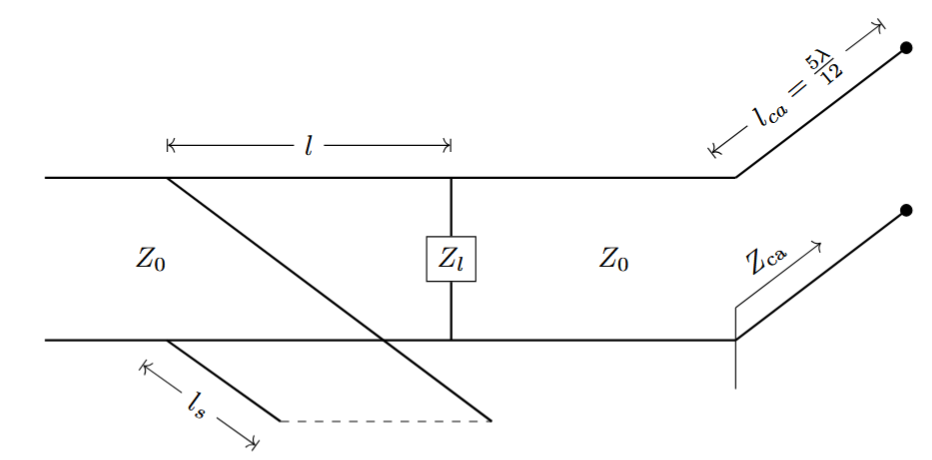
\includegraphics[width=0.5\textwidth]{Auxiliar_8_5}
\end{center}
%%%%%%%%%%%%%%%%%%%%%%%%%%%
\begin{solution}
    \begin{enumerate}
    \item La impedancia $Z_{ca}$ del circuito se calculará con la fórmula $Z_{in}$ para la cual se tiene que $Z_\mathcal{L} = \infty$ y $Z_0 = 50\,\Omega$.
    
    \begin{align}
        Z_{ca} &= \frac{Z_0 (Z_l + j Z_0 \tan(\beta l))}{Z_0 + j Z_l \tan(\beta l)} 
        = Z_0 \frac{1 + \dfrac{j Z_0 \tan(\beta l)}{Z_l}}{\left( \dfrac{Z_0}{Z_l} + j \tan(\beta l) \right)} \tag{89} \\
        &= \frac{ -j Z_0 }{ \tan \left( 2\pi/\lambda \cdot 5\lambda/12 \right) }
        = \frac{ -j Z_0 }{ \tan \left( \frac{5\pi}{6} \right) }
        = \frac{ j \sqrt{3} Z_0 }{3 } \tag{90}
    \end{align}

    \item La impedancia equivalente en la línea de transmisión será la impedancia de circuito abierto en paralelo con la impedancia de la carga, $Z_{eq} = Z_{ca} \parallel Z_L$. En este caso se tiene que $Z_L = (50 - j50)\,\Omega$ y $Z_{ca} = \dfrac{j\sqrt{3}Z_0}{3}$, por lo que para conseguir $Z_{eq}$ se tiene que:
    \begin{align}
        Z_{eq} = \frac{Z_{ca} Z_L}{Z_{ca} + Z_L}
        = \frac{ \dfrac{j\sqrt{3}Z_0}{3}(50 - 50j) }{ \dfrac{j\sqrt{3}Z_0}{3} + 50 - 50j } \tag{91}
    \end{align}

    Esto nos dará como resultado
    \begin{equation}
        Z_{eq} = 83.47 + j37.15 \tag{92}
    \end{equation}
\end{enumerate}
\end{solution}
%%%%%%%%%%%%%%%%%%%%%%%%%%%
\end{questions}
\newpage
%%%%%%%%%%%%%%%%%%%%%%%%%%%

\end{document}